\chapter{Mon stage}
\label{sec:unchapitre}

Lorsque j'ai répondu à l'offre de stage, il avait été initialement prévu que je produise une newsletter ainsi que trois vidéos sur trois APIs différentes qui sont :

\begin{itemize}
    \item Gat'Ape/Okapi
    \item Zbus
    \item Valkey
\end{itemize}

Cependant, aux vues de l'avancement de mon travail et de l'intérêt suscité par les vidéos produites, j'ai accepté de travailler sur trois autres projets :

\begin{itemize}
    \item Explication des difficultés liées à la création et à la publication d'APIs avant l'arrivée du cloud au sein d'Orange
    \item Présentation des avantages du travail en DevOps
    \item Promotion de PnS.com
\end{itemize}



Les vidéos traitant des APIs se devaient d'être vulgarisées et simples à comprendre étant donné qu'elles pourraient être destinées à un public très vaste. Chaque vidéo se doit d'être compréhensible par un programmeur ou un manager par exemple. La principale difficulté est de devoir vulgariser un maximum tout en gardant des précisions pour qu'elles restent pertinentes pour les personnes les plus techniques. La diffusion de ces vidéos pourra servir à montrer les dernières avancées au sein de la SDFY, ou encore pour promouvoir un produit, ou le proposer à des clients en tant que nouvelle solution. \\

En revanche, l'approche pour les 3 autres vidéos est totalement différente, elles s'adressent à un public ciblé : l'une pour le comité de direction\textit{(cf 2.7)} et l'autre pour le comité d'investissement. \textit{(cf 2.8)} et ont principalement un but promotionnel. Chacune de ces deux de ces vidéos ont été réalisées pour un événement particulier. Pour la première la visite du comité de direction et la seconde en vue d'être intégré à une demande de financement. \\



\section{Style de vidéo et choix du logiciel}
Comme précisé dans l'introduction, mon stage est la reprise en mains d'un projet de série de vidéos ayant été commencées par un prestataire externe. La première vidéo avait été faite en scribing, sorte de présentation sur tableau blanc animé avec une main tenant un crayon qui va dessiner les éléments. J'ai volontairement choisi de ne pas réutiliser ce style car il peut s'avérer très répétitif et ennuyeux sur le long terme.

\begin{figure}[htp]
  \centering
  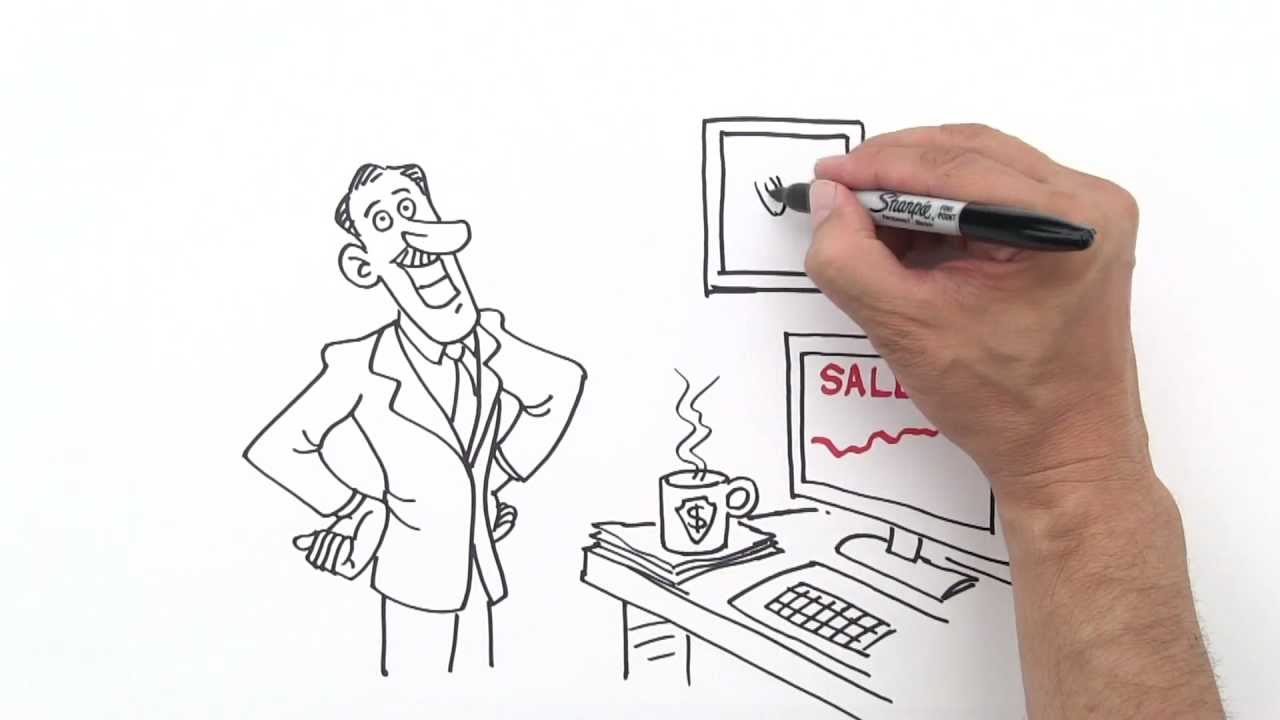
\includegraphics[width=15cm]{images/scribe}
  \caption{Exemple d'une vidéo de type scribing.}
  \label{scribe}
\end{figure}

J'ai opté pour un thème minimaliste afin que les spectateurs ne se perdent pas dans les détails, Un fond blanc ou gris clair et des illustrations issues du site de la marque. De cette manière j'étais sûr de respecter les conditions de la charte graphique, à savoir, au mois 20\% de couleur orange sur les illustrations ainsi que les couleurs et la police de caractères officielle. J'ai dû cependant détourer certaines images, ou en créer d'autres.

En ce qui concerne le logiciel, je me suis servi de Adobe After Effects CC, logiciel que j'avais déjà expérimenté à titre personnel et dont j'ai reçu une formation lors d'un de mes cours du premier semestre. After Effects CC est un logiciel très complet qui permet d'animer des objets de manière précise en ayant la main mise sur tous les paramètres, ce qui permet une création quasiment sans restriction dans un environnement dans lequel j'avais déjà des repères.


\begin{figure}[htp]
  \centering
  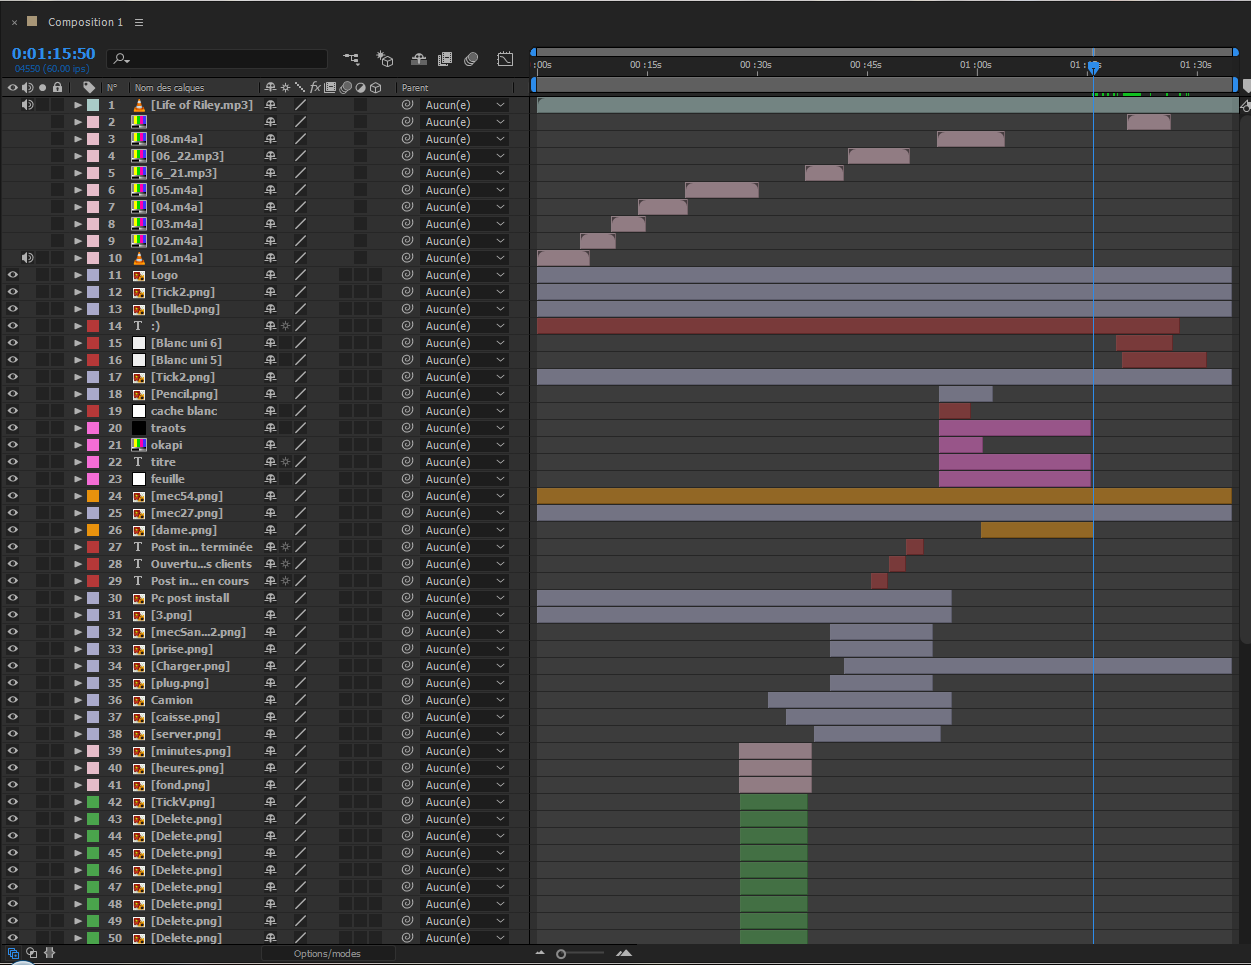
\includegraphics[width=15cm]{images/comp1.png}
  \caption{Fenêtre de prévisualisation de After Effects.}
  \label{ae1}
\end{figure}




\section{Organisation}
Le processus de création de chaque vidéo est découpé en plusieurs phases qui ont toujours lieu dans cet ordre :\\

Si la vidéo était un projet prévu à l'avance, ce qui était le cas pour les trois vidéos traitant les APIs, je commençais par lire de la documentation pour me renseigner sur ce que propose le produit et son utilité.\\

Avait ensuite lieu une réunion avec le chef de projet du sujet de la vidéo ainsi qu'une ou deux autres personnes également concernées (programmeur, graphiste). Lors de cette réunion, je cherchais à comprendre les points importants à développer dans la vidéo ainsi que les messages à faire passer. Si besoin, je demandais également des précisions sur le produit. Une fois les idées et les messages principaux réunis, nous faisons ensemble le tri pour ne garder que les idées les plus pertinentes pour le public ciblé.\\





\begin{figure}[htp]
  \centering
  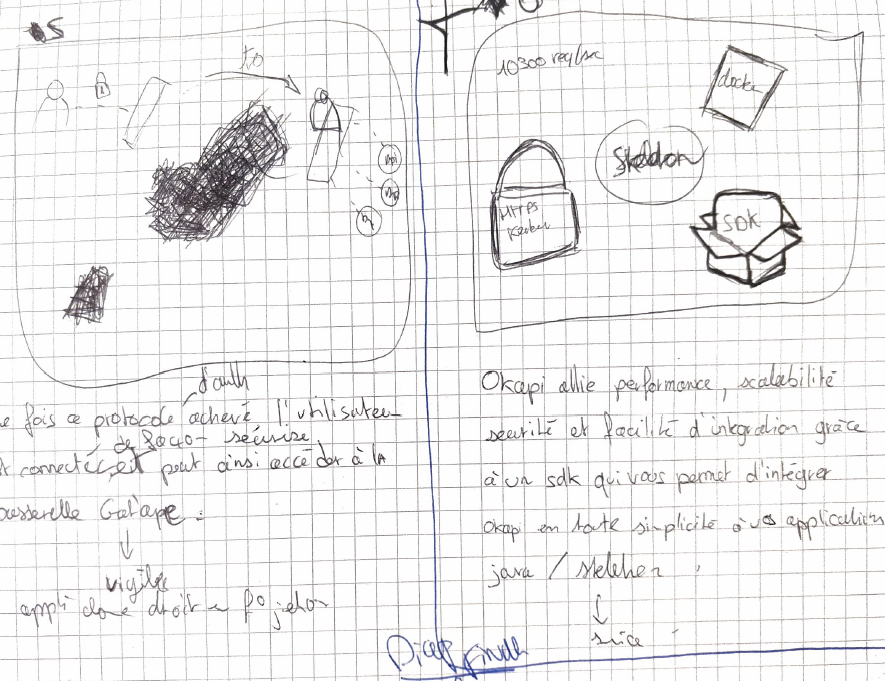
\includegraphics[width=15cm]{images/sb/sb1}
  \caption{Une page du storyboard de la vidéo Gat'ape/Okapi.}
  \label{sbzbus}
\end{figure}




Lorsque le choix est définitif et approuvé par tout le monde, je travaillais sur un storyboard et un script qui permettent de se rendre compte de la mise en page et du texte énoncé. 


Une fois ces deux éléments achevés, je les transmettais aux personnes présentes lors de la réunion pour avoir leurs retour et impressions. S'il y avait des modifications majeures qui nécessitaient une nouvelle phase de vérification, je renvoyais de nouveau le storyboard et le script.\\


Une fois le script validé, je pouvais commencer la création de la vidéo via After Effects en animant les éléments prévus au storybaord pour garder un ensemble dynamique. J'ai optimisé la mise en mouvement les éléments importants sans trop animer la totalité pour que le spectateur puisse se concentrer sur la future voix off. Une fois les animations terminées, j'enregistrais la voix off en lisant le script préalablement écrit puis je la synchronisais avec les animations. Pour finir, j'ajoutais une musique de fond, pour combler les blancs de manière conviviale.\\

Une fois ceci fait j'envoiyais ce pilote aux personnes concernées en attendant leurs remarques éventuelles. S'il y avait besoin de modifier des parties, je le faisais puis leur renvoyais la nouvelle version jusqu'à validation de la vidéo, qui se faisait d'un commun accord entre moi et le chef de projet.


%Avant de développer le contexte et la production de chaque vidéo, je vais d'abord présenter le programme PnS.com et ses différents composants. 

\section{Présentation générale de l'écosystème PnS.com}


PnS.com est une extension de l'ancienne solution de stockage de données à haute performance et disponibilité appelé PnS. Cette extension le rend As A Service (AAS), c'est à dire accessible via internet par le client. L'architecture de PnS.com se divise en quatre parties.

\begin{itemize}
    \item Le backend
    \item Les injecteurs
    \item Le backoffice
    \item Les APIs
\end{itemize}

%%%%%%%%%%
% Schema %
%%%%%%%%%%



Le backend est composé de la base de données Cassandra noSQL, prévue pour stocker un grand nombre de données réparties sur plusieurs serveurs différents. Elle possède donc une haute disponibilité et a un système d'élimination de ponts défaillants qui lui assure une quasi certitude d'accès aux données. Parmi le backend figure aussi Elastic Search qui est un moteur de recherche qui va faciliter la consultation de la base de données, et Omnibus sert de lien entre Cassandra et Elastic Search.\\

Les injecteurs quant à eux, ont le rôle d'envoyer en masse des informations dans la base de données.\\
\begin{figure}[htp]
  \centering
  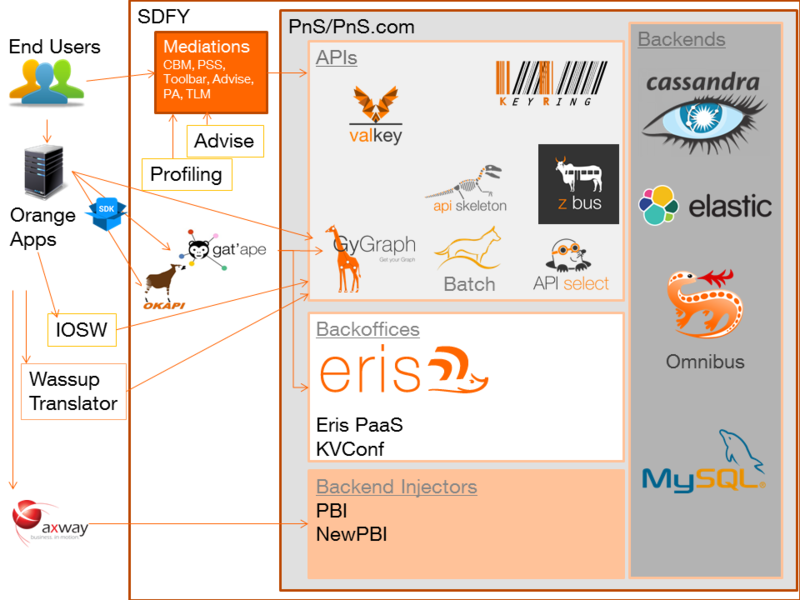
\includegraphics[width=15cm]{images/pns/psn.png}
  \caption{Schéma de l'architecture de PnS.com.}
  \label{pns}
\end{figure}


Le backoffice, et plus particulièrement Eris, l'outil de gestion des flux, permet à un service de type PnS de présenter l'ensemble de ses relations avec ses fournisseurs et ses partenaires. Ses principales fonctionnalités sont de pouvoir rechercher de l'information par mot clef, mais aussi de saisir de l'information et de pouvoir suivre les flux.\\

Enfin, les APIs sont présentes pour ajouter des fonctionnalités à l'écosystème PnS.com. Parmi ces APIs, nous retrouvons Batch, qui va autoriser des injections, Select, qui va permettre de faire des recherches sous forme de texte comme nous le ferions dans un moteur de recherche au lieu d'utiliser les noms des variables. Skeleton, socle pour les APIs, Zbus, dont le but est de transmettre des messages \textit{(cf : 2.3)}, GyGraph qui permet de modéliser une base de donnée sous forme de graphe et Valkey qui fournit le modèle clef/valeur \textit{(cf : 2.4)}.\\

Actuellement, 185 applications se connectent à PnS quotidiennement, ce qui représente 20 000 requêtes/s en lecture et 8 000 requêtes/s en lecture sur la base de données. Ces applications viennent de milieux différents tels que le portail orange.fr, l'espace client ou bien encore le Suivi Conso par exemple. Ces applications viennent chercher : 

\begin{itemize}
\item Des données, les leurs ou bien des données déjà présentes en base
\item Une grande capacité et une scalailité sans impact
\end{itemize}
 
 En effet, PnS dispose de 70TB qui permettent d'absorber les variations de volume de stockage.

\section{Vidéo sur Gat'Ape/Okapi}

\subsection{Contexte}
Gat'ape/Okapi est une API faisant partie de l'écosystème PnS.com qui permet d'exposer, de s'authentifier et de sécuriser les APIs de cet écosystème. Gat'ape et Okapi ont deux fonctions bien distinctes.\\

Okapi est le système d'authentification qui va permettre la connexion aux autres APIs. Il est basé sur le couple Oauth2/Kerberos qui va permettre une identité indépendante à chaque entité tout en offrant un système d'authentification unique (SSO). L'utilisateur pourra accéder à plusieurs applications en ne s'authentifiant qu'une seule fois. Cette authentification repose sur un système de clé secrète et de jeton. Il est à noter que des options de sécurité plus complexes sont aussi disponibles.\\

Gat'ape quant à elle est la passerelle qui va permettre d'exposer les APIs, c'est à dire, de les rendre visibles à d'autres utilisateurs pour qu'ils puissent s'y connecter. Gat'ape va pouvoir offrir un contrôle d'accès et un contrôle de trafic permettant de réguler le flux des utilisateurs. Gat'ape est également responsable  de l'authentification et de la sécurité lors de la consommation par Okapi. En plus de cela, gat'ape est également scalable, c'est à dire qu'elle va pouvoir maintenir son activité et sa performance même lors d'une forte demande.\\

\begin{figure}[htp]
  \centering
  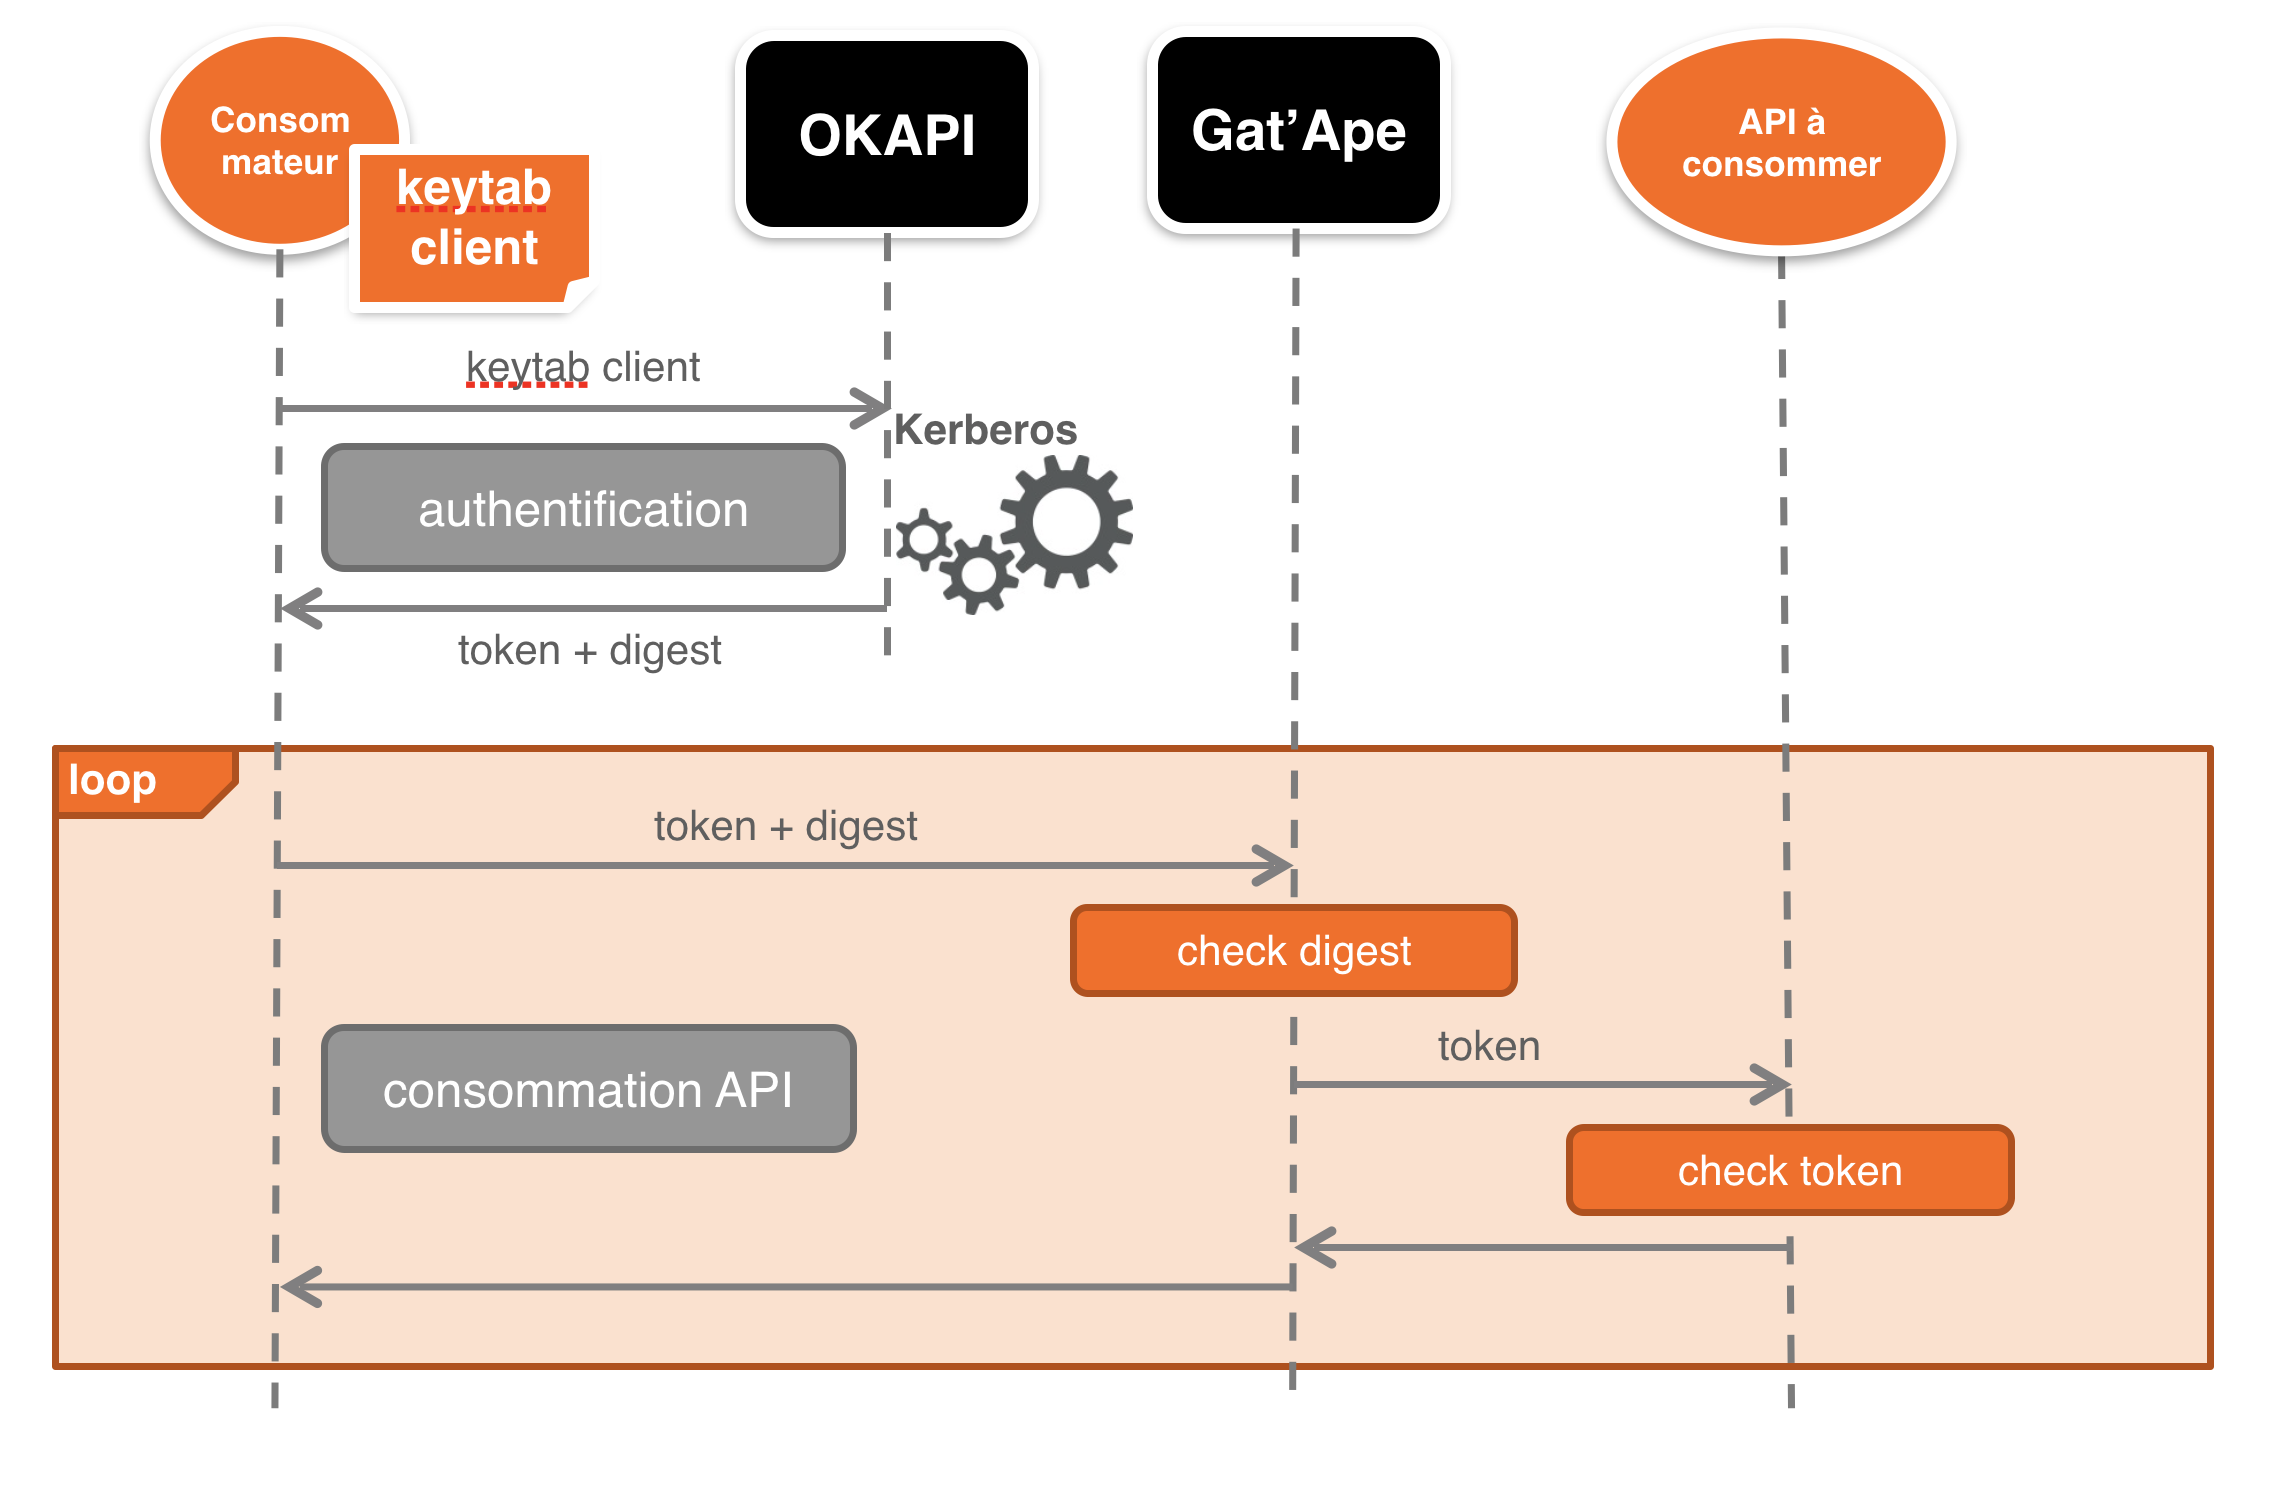
\includegraphics[width=15cm]{images/gao/gao1}
  \caption{Fonctionnement de Gat'Ape/Okapi.}
  \label{gatape}
\end{figure}


Dans les faits la connexion grâce à Gat'ape/okapi se passe comme suit : 
l'application qui vient se connecter possède une clé secrète. Cette clé secrète est envoyée à Okapi. Lors du traitement, Okapi va renvoyer un jeton d'authentification unique au consommateur ainsi qu'un digest. Ceci est la phase d'authentification.  Ce digest est ensuite envoyé du consommateur vers Gat'ape. Si le digest est valide, le consommateur va envoyer le jeton précédemment obtenu vers l'API à laquelle il souhaitait se connecter. L'API va à son tour vérifier le jeton puis le renvoyer ainsi que les informations demandées par le consommateur. Ces informations lui seront transmises via Gat'ape. Si une de ces vérifications de jeton échoue, le protocole recommence un envoi de jeton. L'opération peut ainsi être réitérée un certain nombre de fois sans avoir à se ré authentifier. Cette durée de vie (TTL) est paramétrable.




\subsection{Réalisation}
Avant de commencer la production à proprement parlé j'ai tout d'abord dû lire la documentation relative à cette API pour en comprendre l'utilité et le fonctionnement. Une fois que la fonction et le fonctionnement de cette API m'étaient plus clair, j'ai pris rendez vous avec le responsable solution de cette API. Nous avons fait une réunion dans laquelle je lui ai demandé les points qu'il voulait mettre en avant grâce à la vidéo et les principales innovations qu'apportait Gat'ape/okapi par rapport à l'ancienne solution. Une fois d'accord sur les points à aborder je me suis mis à produire un script et un storyboard qui sont respectivement le texte de la vidéo et les images et animations clefs de celle-ci. Une fois le script et le storyboard finalisés, j'ai de nouveau rencontré le responsable de Gat'ape/Okapi pour les lui proposer. Une fois ces documents validés, j'ai pu me lancer dans la production. \\

Au lancement de la vidéo, les logos de Gat'ape et Okapi arrivent depuis chaque côté de l'écran, présentant ainsi les deux APIs. La partie suivante de la vidéo explique brièvement la fonction générale de Gat'ape/Okapi. Pour cette première partie j'ai voulu expliquer simplement et en quelques secondes à quoi servait Gat'ape/Okapi. Les APIs exposées au travers de Gat'ape apparaissent en premier, pour symboliser le fait qu'elles sont déjà présentes et visibles, puis les consommateurs font leur apparition et ces derniers sont reliés aux APIs via des flèches en passant par le duo Gat'ape/Okapi.\\

Vient ensuite l'explication de l'identification. Le nom du protocole d'authentification, Okapi, apparaît et est décomposé pour expliquer son acronyme. Dans un premier temps le protocole Oauth2 est présenté comme étant le moyen de mise en relation du consommateur avec Okapi,  puis Kerberos est succinctement introduit comme étant un protocole d'identification à base de clés secrètes et de jeton. Kerberos étant crucial et complexe, j'ai choisi de l'expliciter dans la partie suivante de la vidéo autour d'une situation connue de tous, l'accès à une salle de cinéma.\\

Dans un premier temps le spectateur (dans le cas concret : le consommateur) va récupérer au guichet (Okapi) son ticket. Une fois ceci fait, le spectateur doit passer devant l'ouvreur au point d'accès de la salle qui va déchirer le ticket et en garder une partie. Lors du contrôle (l'accès à Gat'ape), il est vérifié que les deux morceaux de tickets vont bien ensemble, si c'est le cas le spectateur peut accéder à sa séance (Le consommateur peut accéder à l'API). Il est ensuite précisé que le ticket a une durée bien définie, une séance dans le cas d'un ticket de cinéma, un Time To Live (durée de vie) paramétrable dans le cas de Gat'ape/Okapi.\\

\begin{figure}[htp]
  \centering
  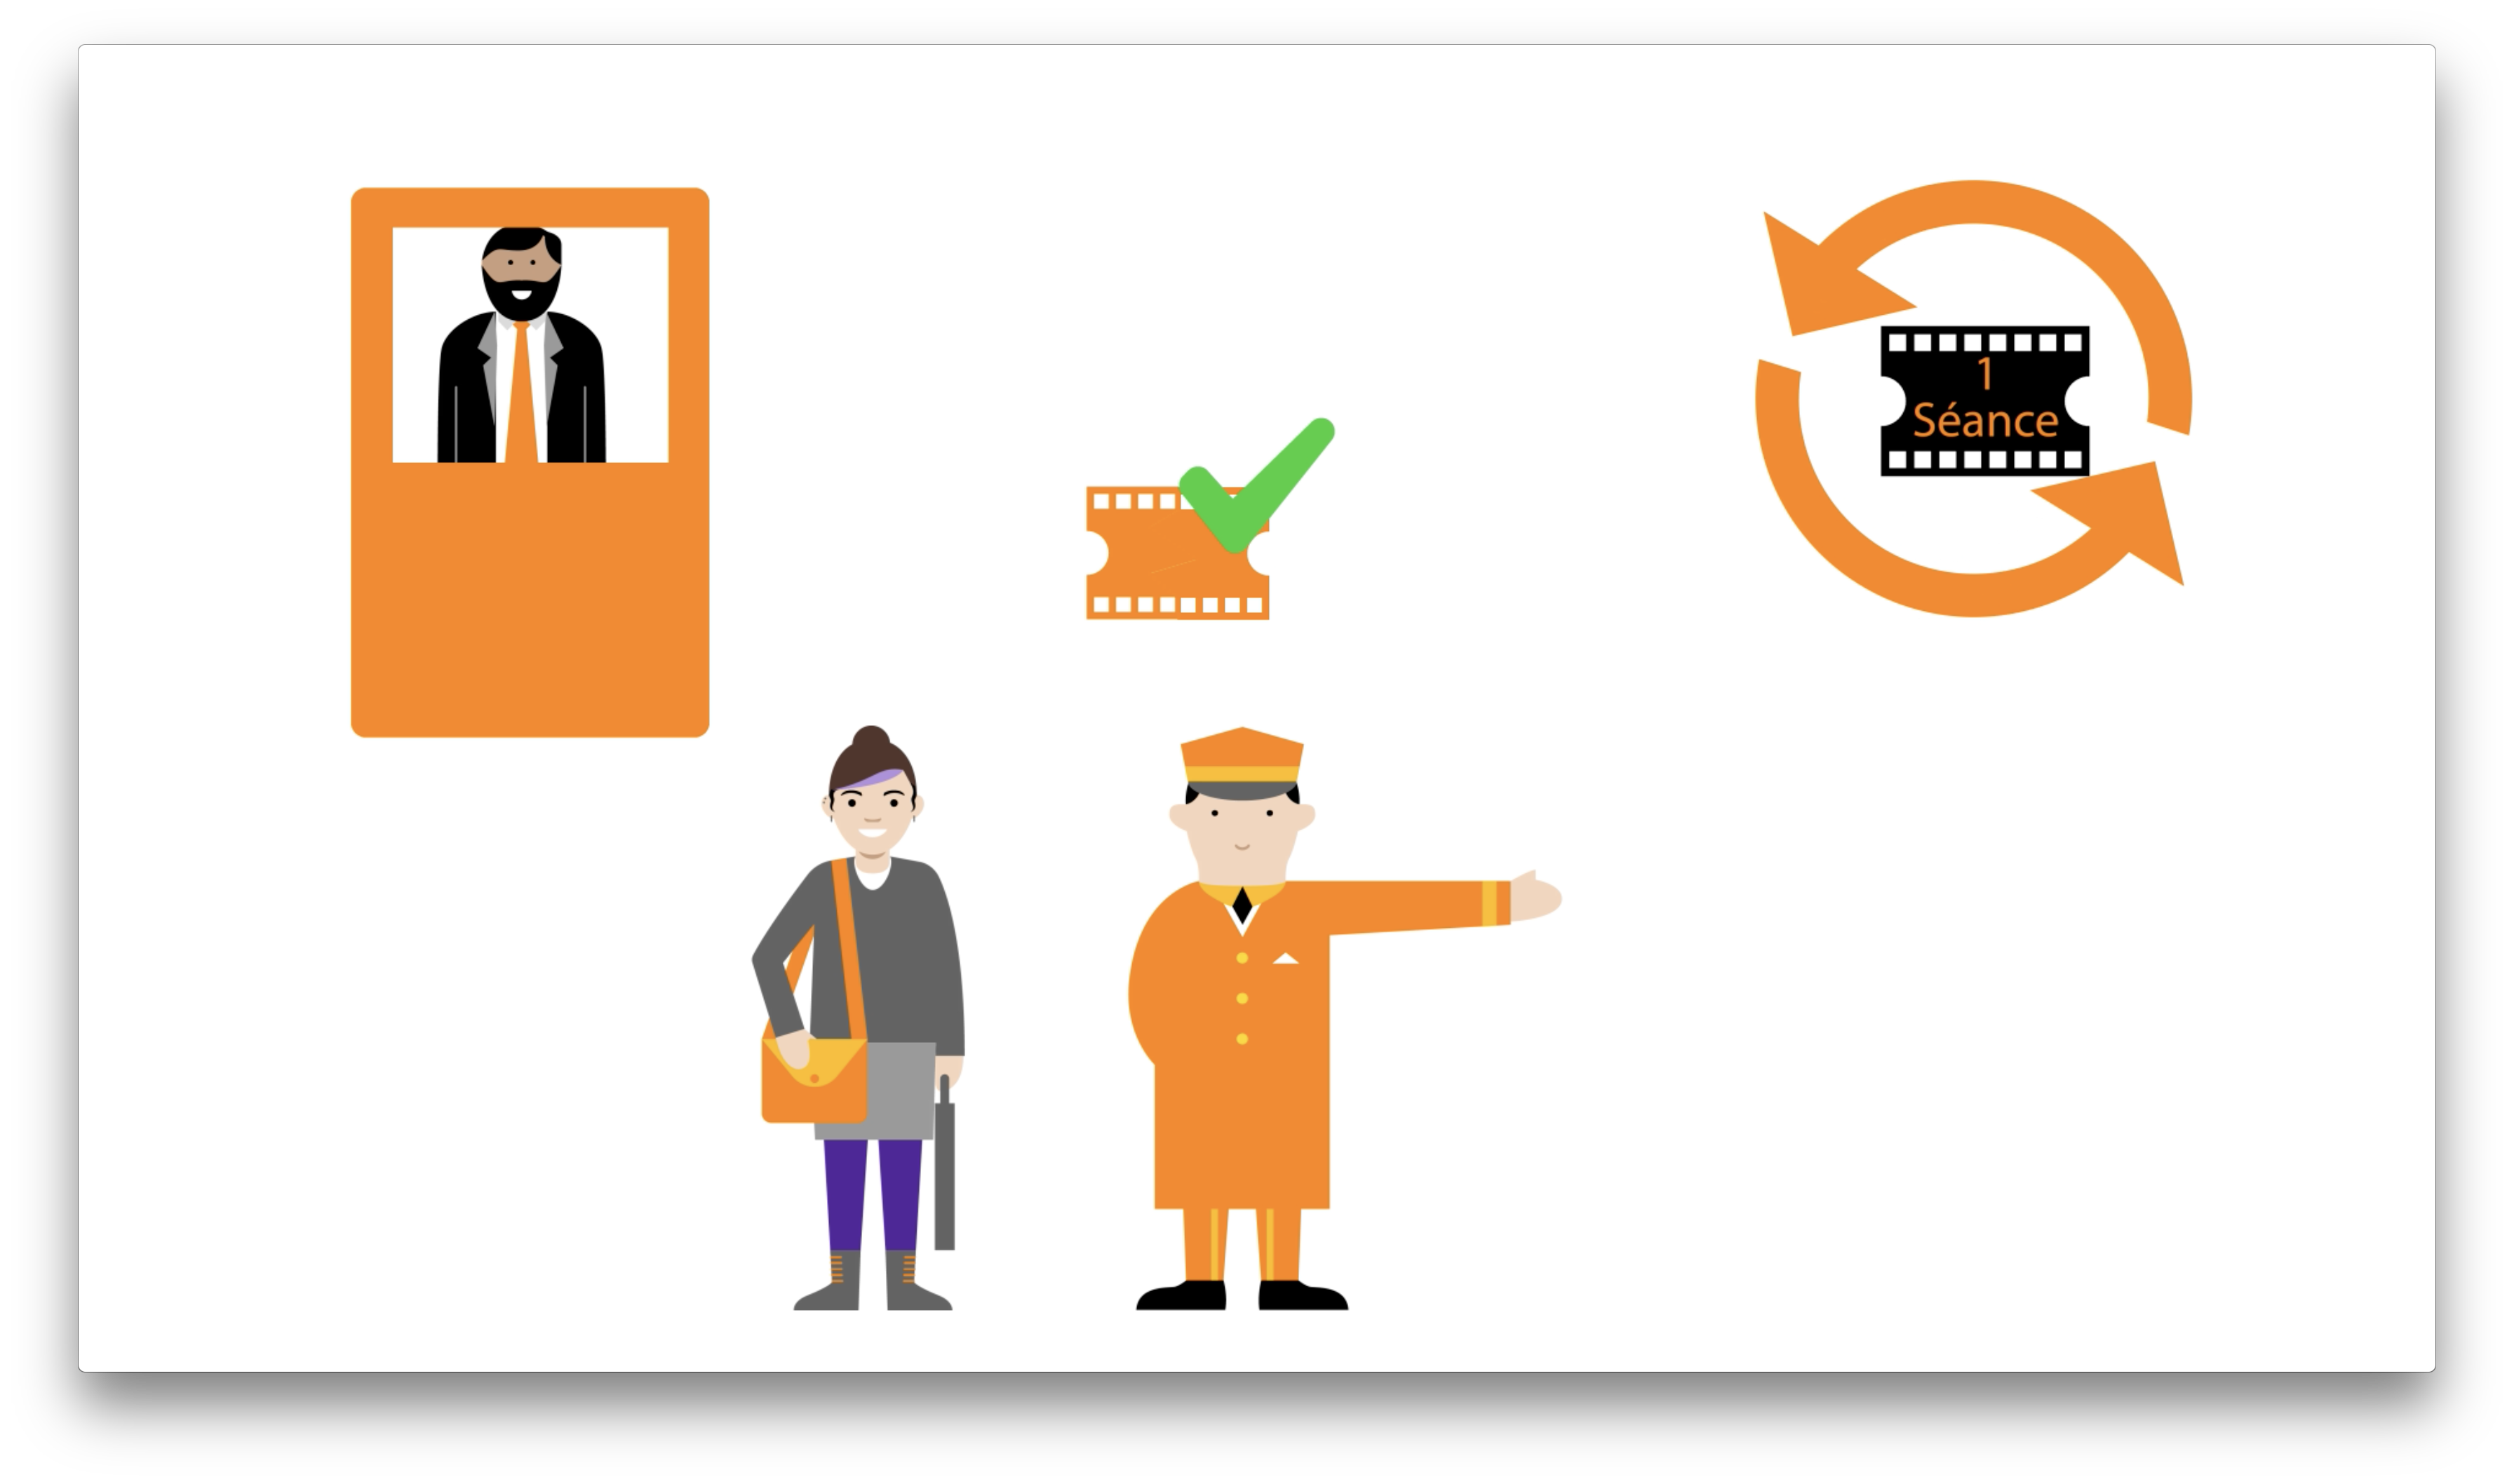
\includegraphics[width=15cm]{images/gao/screenGao}
  \caption{Explication de Kerberos.}
  \label{screengatape}
\end{figure}

Il est ensuite mis en avant les possibilités qu'offre Gat'ape dans la mise en relation entre le consommateur et l'API, tels le contrôle d'accès (qui va permettre d'autoriser ou non l'accès à une API à certains consommateurs) et le contrôle de trafic (qui va permettre de réguler les flux d'accès en fonction de la demande des consommateurs et de la disponibilité de l'API). Pour représenter le contrôle d'accès j'ai choisi d'utiliser des croix rouges et des coches vertes afin de rester simple et compréhensible. J'ai choisi d'illustrer le contrôle de trafic avec des feux tricolores que l'on voit changer de couleur pour symboliser le fait que ce contrôle n'est pas figé et se déroule en continu. La fonctionnalité mise en avant ensuite est la détection d'erreurs et d'anomalies qui est fournie par une autre API intégrée à Gat'ape (représentée par un moniteur qui contient une sorte d'électrocardiogramme qui grandit dangereusement à un moment). Cette anomalie est ensuite entourée en rouge avec un panneau danger, qui représente la détection.\\

Les fonctionnalités mentionnées ensuite sont un surcoût de temps de réponse quasi nul qui n'impacte pas les performances. Une architecture tri site, qui assure  une très haute disponibilité. En effet, si l'un des trois sites venait à subir une maintenance, une attaque ou être indisponible pour une autre raison, il y a deux autres sites qui pourront fournir l'authentification et garantir la sécurité aux consommateurs.\\

Pour éviter que les personnes les moins techniques ne perdent leur attention à la fin de la vidéo, étant donné sa durée, j'ai choisi de faire un rapide résumé de la situation en rajoutant l'information qu'il existe un SDK pour permettre l'intégration facile de Gat'ape/Okapi à son application et qu'il existe un modèle d'API contenant Gat'ape/okapi prêt à l'usage pour les personnes souhaitant développer une API. Dans la dernière séquence, sont indiqués les liens vers la documentation et le mail de l'équipe en charge pour les personnes souhaitant avoir plus d'informations à ce sujet. 



\section{Vidéo sur Zbus}

\subsection{Contexte}
Zbus est une API permettant le transfert de messages au fil de l'eau entre les applications du SI. Zbus a pour but de faciliter et standardiser l'alimentation de Push@voo, qui est la plate forme permettant d'envoyer les notifications,  comme par exemple le nombre de mails non lus. L'API Zbus fonctionne sur un modèle de publish/subscribe : les messages sont classés par catégories auxquelles s'abonnent les récepteurs. Les messages sont donc en attente active ou "polling" et ne sont délivrés qu'une seule fois. Chaque récepteur a sa propre file d'attente qui sera donc remplie avec les messages dont les catégories l'intéressent dans l'ordre d'arrivée.  


\subsection{Réalisation}

Une fois d'accord sur le storyboard avec le responsable de l'API, j'ai commencé la réalisation. Comme pour la vidéo précédente, l'ouverture se fait avec le logo de l'API Zbus qui arrive à l'écran puis disparaît. Lors de la séquence suivante, la fonction de l'API est résumée très brièvement en tant que la composante qui permet l'envoi de notification, ce qui est, entre autre, une de ses fonctions. J'ai choisi cette facette de Zbus car elle est très facilement compréhensible et visualisable. L'animation par dessus la voix off est donc une enveloppe qui arrive et une notification ronde qui apparaît pour signifier qu'un nouveau message est arrivé.\\

Vient ensuite les explications sur le fonctionnement de l'API. Pour symboliser le fait que les récepteurs s'abonnent au fil de messages, ils sont reliés par un trait à l'émetteur en forme de nuage. On voit ensuite à quelles catégories de messages chaque récepteur s'est abonné sur son écran. Ici pour des raisons de simplicité, les catégories de messages sont représentées par trois couleurs : bleu, rouge et vert. Un des récepteurs est abonné aux trois catégories de messages, un autre à seulement deux catégories et le troisième n'est abonné qu'à la catégorie bleue. Ensuite, la file d'attente de chaque récepteur apparaît à côté de lui et l'émetteur commence à envoyer des messages. 


\begin{figure}[htp]
  \centering
  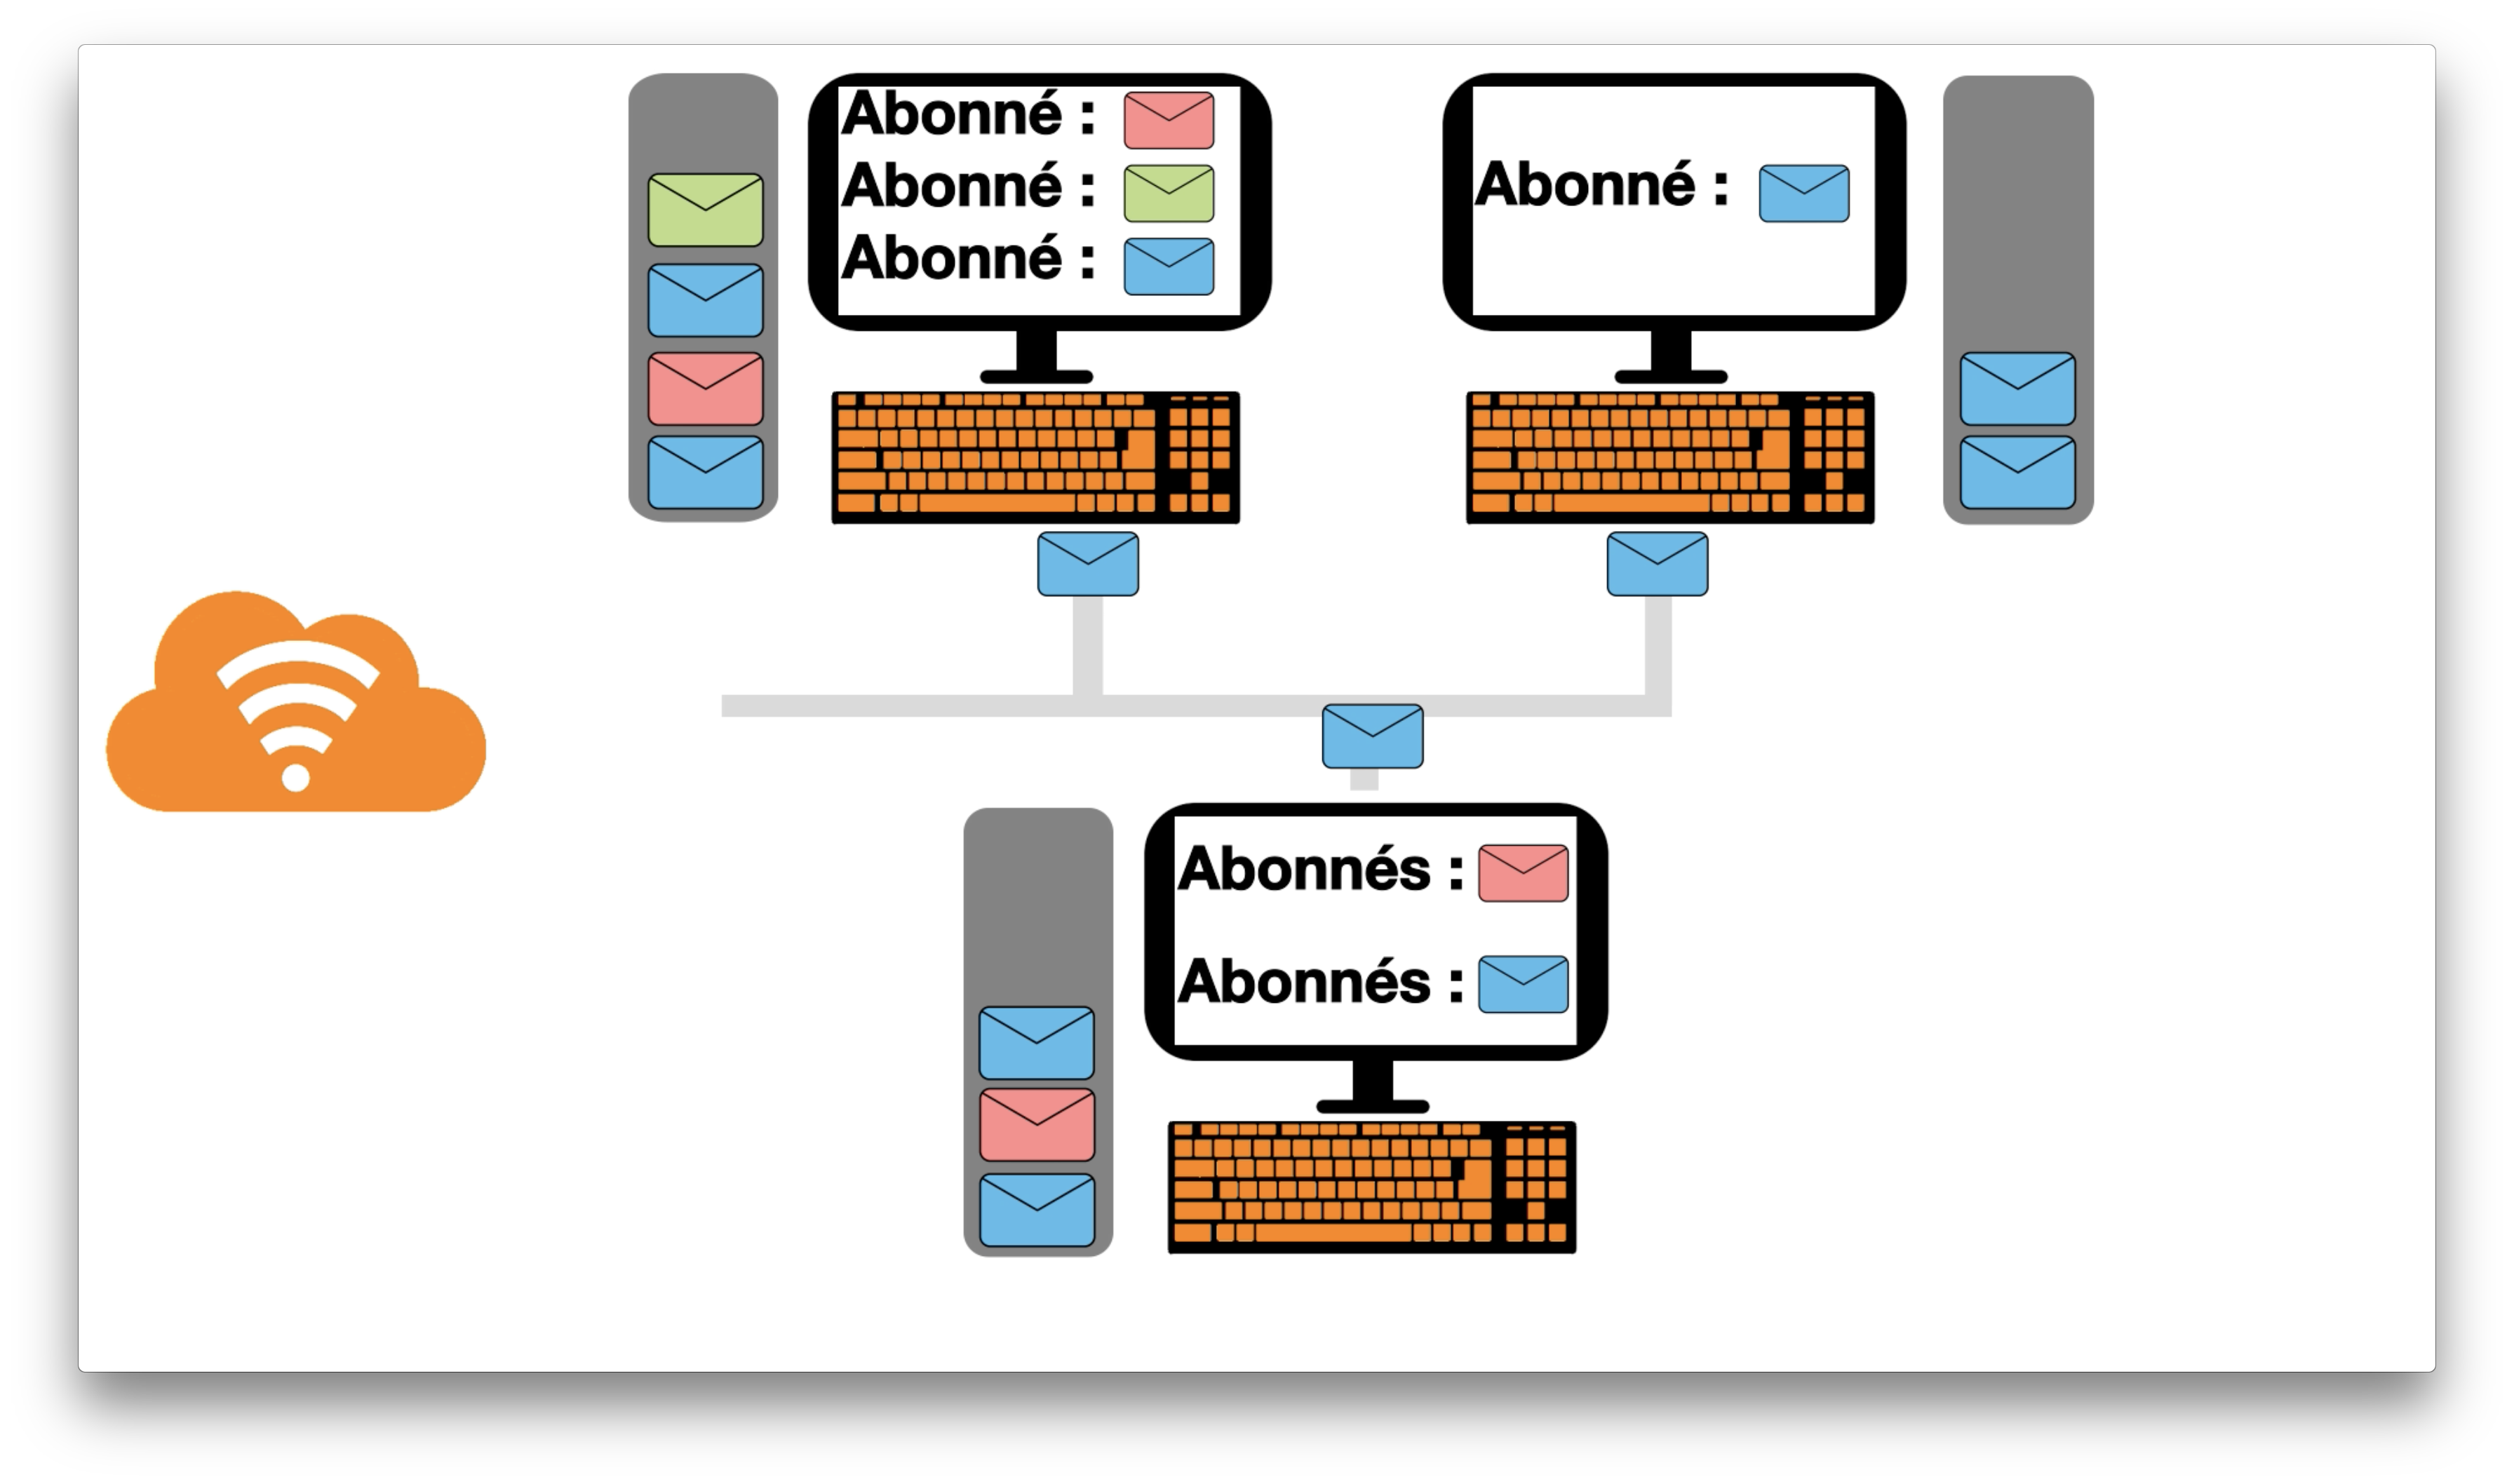
\includegraphics[width=15cm]{images/zbus/screensbus.png}
  \caption{Les files d'attentes dans Zbus.}
  \label{screenzbus}
\end{figure}


Un message est émis une seule fois puis sera intercepté par les récepteurs abonnés à cette catégorie puis stocké dans leur file d'attente en attendant d'être traité. À la fin de cette séquence, chaque récepteur a bien dans sa file des messages correspondant à ce dont ils s'était abonné.\\

La séquence suivante évoque les types de fichiers qui peuvent être échangés via Zbus. L'animation correspond tout simplement au changement de mot au moment de la parole.\\

Puis vient une animation expliquant les avantages de Zbus qui sont sa facilité d'utilisation et sa sécurité. Les logos descendent depuis un trait situé entre une fenêtre d'application et le logo de Zbus. Ce logo va ensuite se décaler et cohabiter à l'écran avec le logo de Push@voo. Une enveloppe va circuler de Zbus vers Push@voo puis des notifications rondes vont ensuite apparaître, expliquant une nouvelle fois que Zbus fonctionne de pair avec Push@voo pour permettre l'envoi de notifications.\\

Enfin, nous retrouvons une séquence classique qui contient les liens intranets vers la documentation et le mail de l'équipe de Zbus.


\section{Vidéo sur Valkey}

\subsection{Contexte}
Valkey est une API permettant la liaison entre la donnée et la base. Elle permet de stocker la donnée en base ou bien de la rechercher afin de la fournir au consommateur. Cette API permet deux types de stockages différents :\\
\begin{itemize}
\item Le stockage clef-valeur
\item Le stockage clef-colonne\\
\end{itemize}

Le stockage clef-valeur est le mode  de stockage classique du noSQL sur un modèle simple: à une valeur correspond une clé. Un modèle simple, qui permet une forte évolutivité car il n'est pas typé. Ce type de stockage est utilisé sur les données de faible à moyen volume, pour garder une vitesse de recherche élevée\\

En cas de volume plus important, Valkey peut fournir un modèle de stockage clef-colonne plus rapide. Au cours d’un enregistrement, une colonne peut être créée, sachant que le nombre de colonnes peut varier d’un enregistrement à un autre, évitant les colonnes de valeur NULL.\\


\subsection{Réalisation}

Dans un premier temps, il est montré au spectateur que sur une même page, les données peuvent venir de plusieurs endroits différents, et que ces données doivent êtres acheminées depuis la base de données vers l'application via Valkey\\

Pour la réalisation de la partie explicative, j'ai d'abord mis en image la différence entre les deux types de stockage via des représentations simples des bases de données grâce à des exemples assez parlant comme le stockage des factures de plusieurs clients. Le même jeu de données est traité dans chacun des modes de stockage afin que le spectateur puisse comprendre les différences.\\

Au moment où j'écris ces lignes, la réalisation de cette vidéo n'est pas terminée, je ne peux donc pas vous expliquer en détail les séquences. Cependant, il est prévu d'ajouter les éléments qui font la force de cette API comme sa scalabilité, sa performance et sa facilité d'intégration 



\section{Le cloud chez Orange (Comité de direction)}
\subsection{Contexte}
Le 12 juin 2016, Koen Vermeulen, CIO d'Orange ainsi que son comité de direction sont venus sur le site de Sophia-Antipolis dans le but de voir les avancements du cloud et comment celui-ci pouvait impacter la totalité d'Orange et pas seulement les développeurs axés sur les nouvelles technologies comme c'est la cas à la DFY. Un créneau de démonstration a donc été réservé pour une équipe qui devait montrer les différentes étapes avant et après l'arrivée du cloud pour un développeur qui souhaite créer une application se connectant à la base de données.\\

J'ai donc été missionné pour la première partie de cette intervention en ayant pour but de "produire une vidéo de moins de 3 minutes expliquant le côté laborieux pour un développeur de déployer une application depuis avec les étapes de demande de machines, flux, connections au backend".\\

Cette vidéo fut suivi d'une démonstration d'un déploiement d'une API en obtenant automatiquement les identifiants de connections.

\subsection{Réalisation}
Avant de réaliser le storyboard, j'ai dû rencontrer les deux développeurs qui s'occupaient de la démonstration programmée. juste après ma vidéo dans le but de savoir sur quels points je devais appuyer afin que leur démonstration fasse bien contraste avec la situation précédente. Les points qui sont ressortis sont

\begin{itemize}
    \item Le temps à attendre avant la mise en service
    \item Les formulaires à remplir manuellement qui transitaient de main en main
    \item La nécessité de passer par des services externes
\end{itemize}

J'ai donc construit la vidéo autour de ces idées principales tout en racontant une histoire. La vidéo s'ouvre sur un programmeur qui a une idée d'application mais qui ne peut pas être implémentée par faute de serveurs. Cette personne va donc demander à son manager si elle peut en obtenir un. Pour ce faire, le manager va passer commande. Ici on retrouve le temps perdu. Il a été mis en image par la symbolique des aiguilles de l'horloge qui tournent vite ainsi que les jours qui défilent dans le calendrier. Une fois le serveur livré, un autre point d'intérêt est abordé, il s'agit ici de l'intervention d'une équipe qui va brancher, configurer et paramétrer les serveurs. Enfin, la partie administrative est mise en image avec le côté redondant d'un papier qui va circuler de main en main avant d'être enfin validé. La vidéo se termine sur la personne du début qui peut enfin mettre en place son application.\\

Cette fin permet à l'équipe de démonstration de pouvoir enchaîner et de faire contraste avec le temps nécessaire avant mise en place du cloud, et les quelques minutes de déploiement de la démonstration.

\begin{figure}[htp]
  \centering
  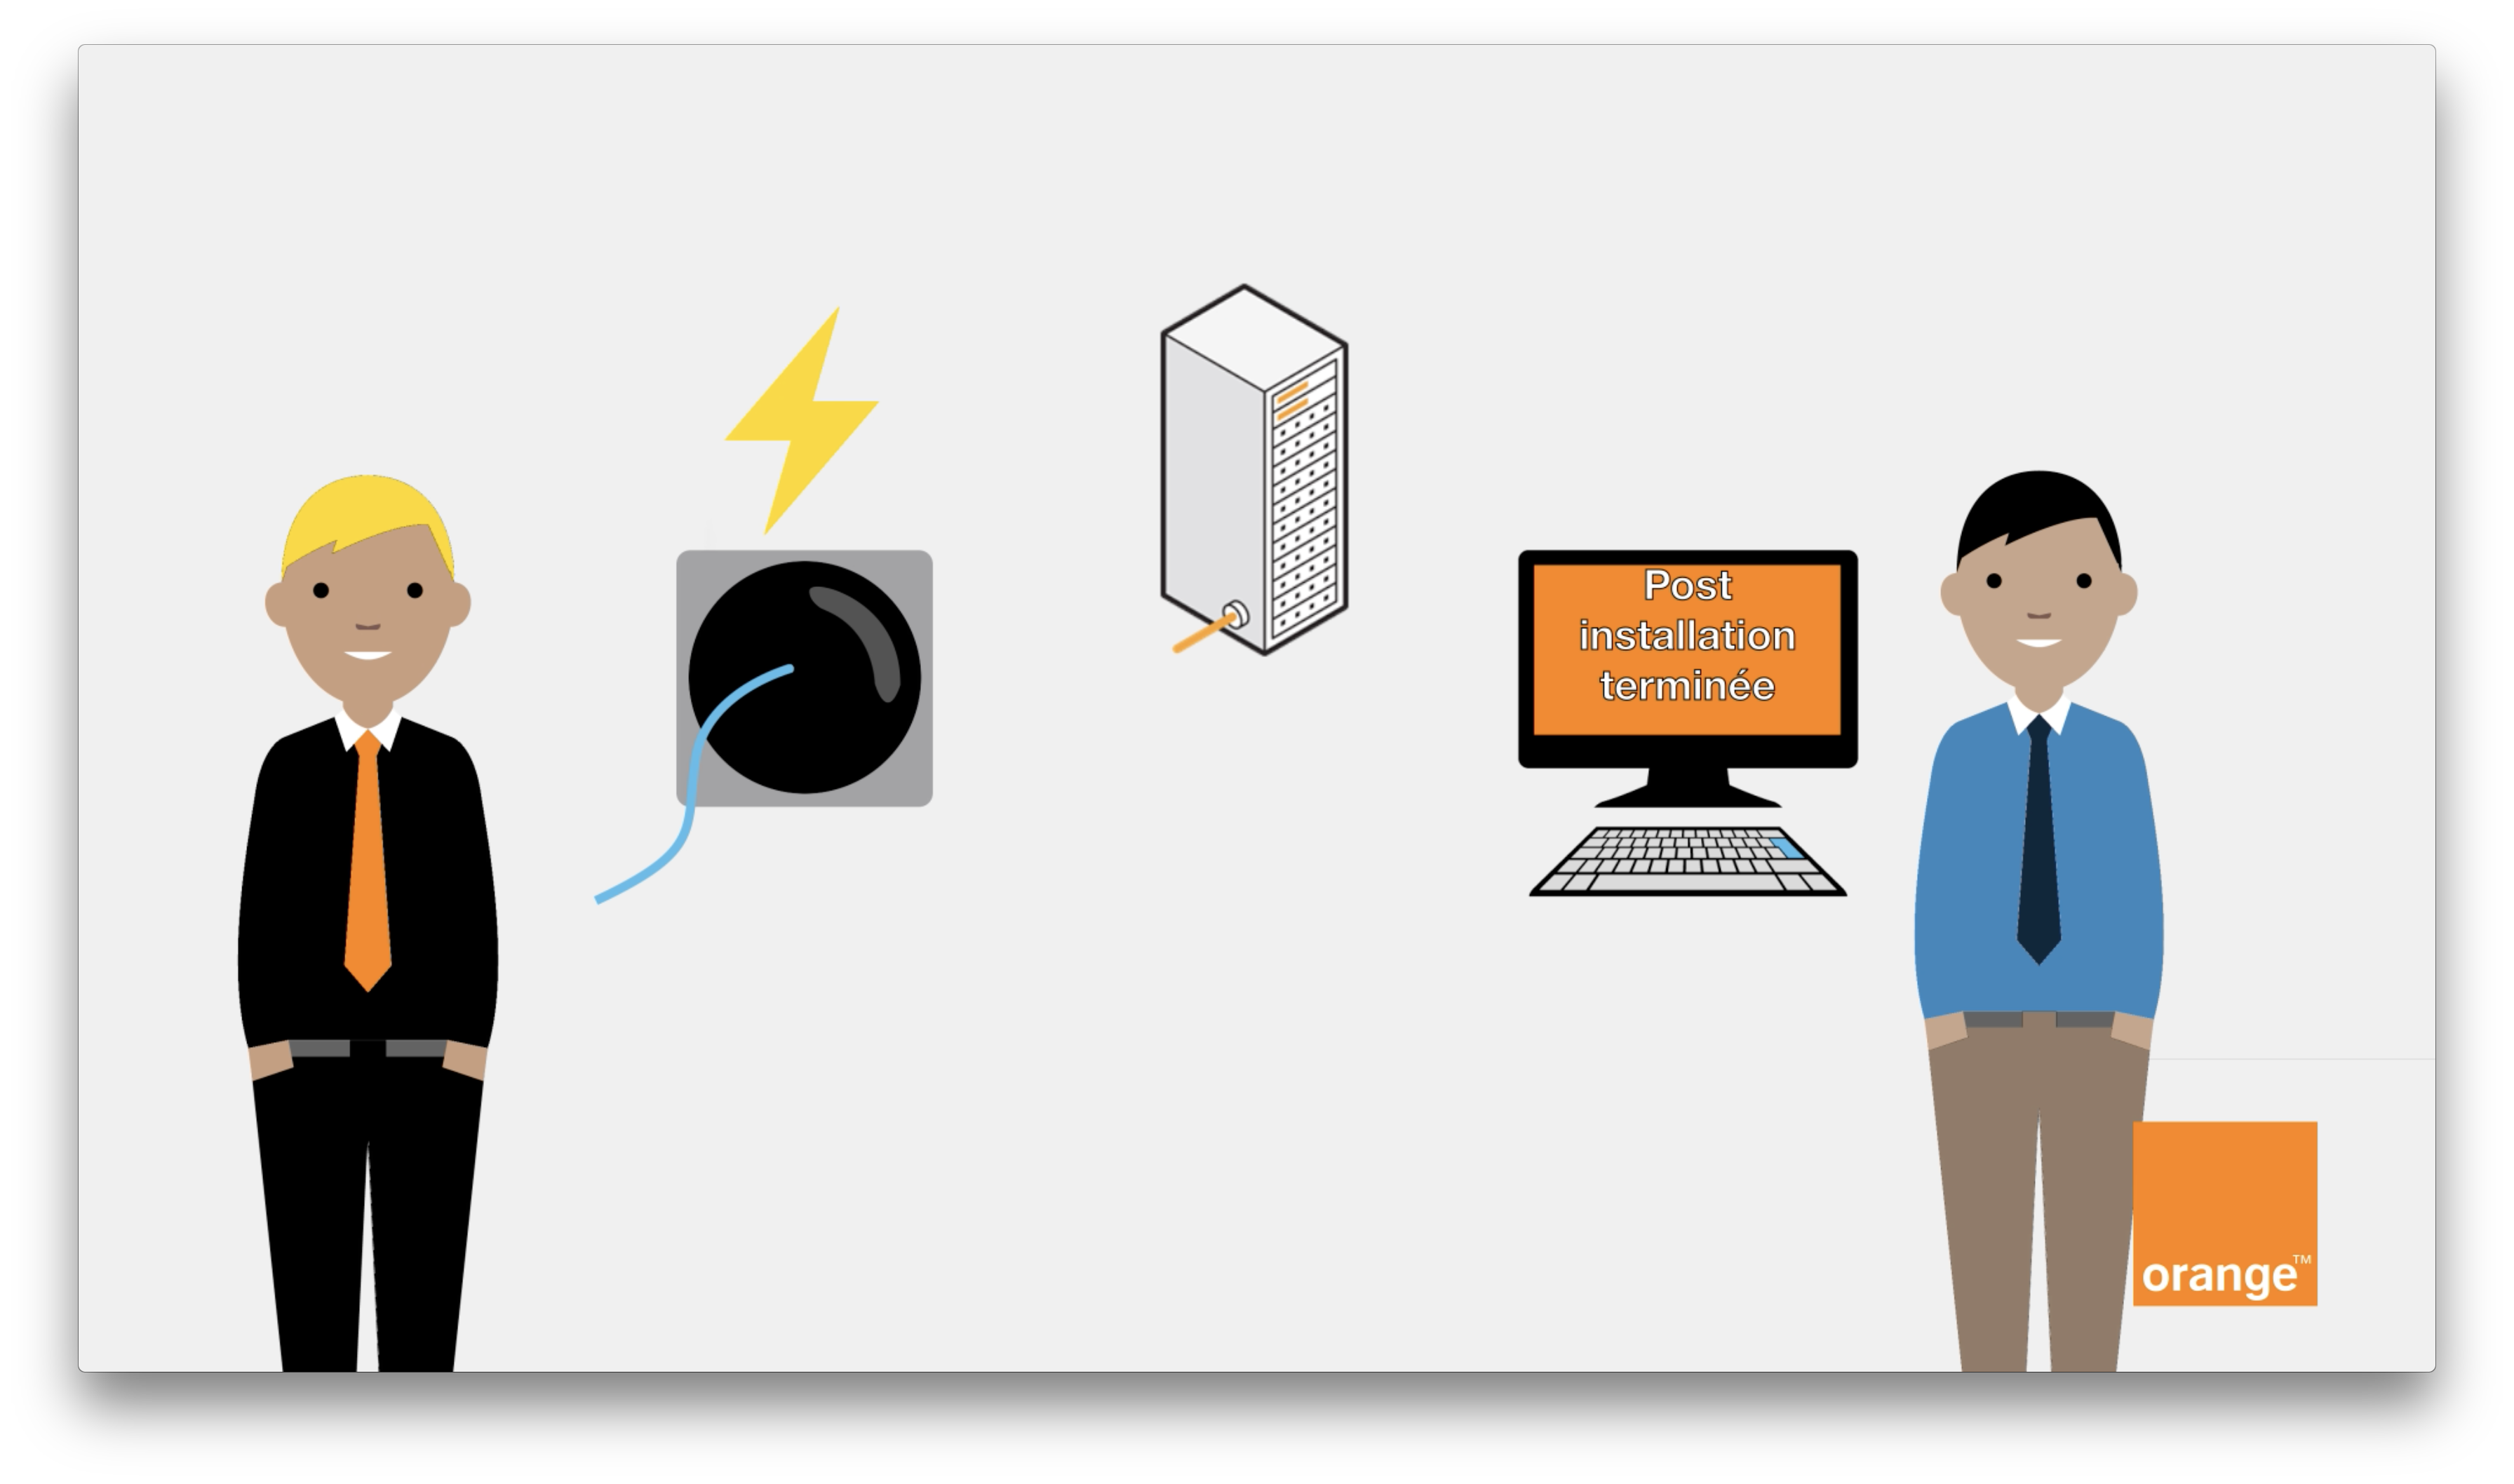
\includegraphics[width=15cm]{images/cd/cd.png}
  \caption{Les étapes de l'installation avant la mise en place du cloud.}
  \label{comite}
\end{figure}



\section{Présentation de PnS.com (Comité d'investissement)}
\subsection{Contexte}
Peu après mon départ, la DFY passera devant un comité d'investissement dans le but de récolter de l'argent pour financer PnS.com. Lors de cette présentation, la direction souhaitait ajouter une note plus ludique et changeante que les habituels diaporamas et ont donc demandé une vidéo pour rappeler les innovations et promesses de PnS.com. Cette vidéo se doit donc d'être assez courte et concise. Les points importants à aborder étaient : 
\begin{itemize}
\item Le stockage des données
\item Les promesses de performance
\end{itemize}




\subsection{Réalisation}
La vidéo devait faire moins de 3 minutes, j'ai dû faire des choix quant à quels éléments intégrer ou non. Dans un premier temps j'ai choisi de montrer les différences entre le traitement des données sans PnS.com et avec. Dans le premier cas, nous avons un administrateur de bases de données par projet et une fois injectées, les données sont dupliquées avant de pouvoir être consultées. De plus en cas de déplacement des données ou augmentation du nombre de requêtes par secondes des coûts supplémentaires pouvaient s'ajouter, sans compter les coûts des licences. En vidéo, ceci est représenté par une écosystème de bases de données dans lesquelles transitent des points représentant les données et illustre par leur déplacement et réplication les points énoncés ci dessus.\\

Avec PnS.com, il n'y a qu'une seule base de données et une fois injectées, les données sont récupérables sans duplication. De plus, PnS.com utilise des éléments open source, ce qui permet une diminution des coûts, représentés par un symbole euro et une flèche pointant vers le bas.\\

Pour les points suivants, PnS.com a été symbolisé au centre et chaque élément vient se greffer autour au moment de l'énonciation de ses différents atouts comme la sécurité ou la scalabilité par exemple.


\section{Présentation du DevOps}


\subsection{Contexte}

Après avoir visionné ma vidéo sur Gat'ape/Okapi, une personne \textbf{PRECISER LE ROLE OMG} est venue me proposer de réaliser un projet à propos du DevOps, qui correspond au mélange des tâches qu'effectuent les équipes d'une entreprise chargée du développement des applications (Dev) et de l'exploitation des systèmes (Ops). Cette personne avait réalisé un an plus tôt une présentation dans laquelle elle expliquait le développement du DevOps au sein d'Orange et en quoi celui-ci était bénéfique. Elle rencontrait cependant un problème, le support de cette présentation était un fichier dans lequel les informations étaient résumées de façon succinte et étaient dans la majeure partie des cas insuffisantes pour pouvoir comprendre l'essentiel du propos. La conférence avait cependant été filmée, mais l'intervention durait une vingtaine de minutes, ce qui demande une longue période d'attention. L'enjeu de ce projet était de produire une vidéo qui se suffirait à elle même, assez courte et suffisamment précise pour reprendre les points de la présentation.


\subsection{Réalisation}
La principale différence avec cette réalisation c'est que le storyboard était déjà défini, il suffisait de reprendre les étapes décrites lors de la présentation. Il m'a aussi été demandé de réutiliser les images du précédent support. Celles-ci ayant été créées spécifiquement par un graphiste. Notre première réunion était donc composée de la personne ayant réalisé la présentation et effectué la demande de vidéo et du graphiste. Ce dernier m'a fournit les éléments graphiques utilisés dans la présentation ainsi que certains modèles sous format vectoriel dont j'avais déjà entrevu des modifications à apporter.\\

J'ai ensuite eu une réunion \textbf{LA NOMMER ET DONNER SON NOM AVANT} avec la personne de la présentation pour travailler le texte de la voix off, car elle m'avait préalablement envoyé un prototype de texte qui durait environ sept minutes à la lecture, ce qui était bien trop long. Nous avons donc extrait ensemble les messages importants à véhiculer et nous avons dû éliminer beaucoup de petits détails tels que des chiffres qui n'apportaient pas directement des informations liées au DevOps. Garder uniquement les informations concrètes fut la partie la plus complexe de la pré-production. Nous avons fini par garder environ 5 minutes de texte essentiel sur les 30 minutes de la présentation.\\

Une fois cette phase terminée, la voix a été enregistrée par la personne en anglais et en français puis m'a été transmise. Disposant donc des illustrations, de la voix et de la présentation, il ne me restait plus qu'à retranscrire cette dernière sous forme d'une vidéo dynamique. Il ne me restait plus qu'à faire les animations. Pour réaliser la plupart de  celles-ci, j'ai dû découper les images fournies pour pouvoir les animer partie par partie afin de créer des effets d'apparition au fur et à mesure de la progression du texte. 


\section{Newsletter}

Il m'a également été demandé de mettre en forme une newsletter pour résumer les dernières nouveautés de la DFY. Les thèmes présents ont tout d'abord été choisis par Olivier, mon responsable au sein de la DFY. Nous avons ensuite contacté les différentes personnes pour récolter une petite interview afin de connaître les innovations de leurs solutions pour que nous puissions les mettre en avant dans la newsletter.\\

J'ai ensuite commencé à travailler sur un modèle qui, suite à plusieurs itérations avec
l’équipe de designers et de la direction, est devenu le modèle présenté en annexe \textbf{NUMERO D'ANEXE}. L'idée était de proposer une newsletter moderne, agréable et qui donnait envie d'être lue, d'où les choix de mise en page originaux et ludiques.



%%% Local Variables: 
%%% mode: latex
%%% TeX-master: "isae-report-template"
%%% End: 